% !TeX spellcheck = en_US
\documentclass[titlepage]{article}
\usepackage{pacco}
	\makeindex
\begin{document}
	\title{Probability theory notes}
	\author{Kotatsu}
	\date{\small TOALDO COL \textbf{CAZZO} CHE DIVENTI ORDINARIO}
	\maketitle
	\begin{preface}
		This document stems from the fact that I just seem unable to pass the Probability Theory exam for the life of me. I regret with every ounce of my being the fact that I enrolled to the Stochastics and Data Science master degree a year ago. Since dear Professor Toaldo never really thrilled me with his insightful lectures about this delightful topic, I resorted to watch the old lectures by Professor Polito, who at least seems to know the subject and to be determined to explain it.\\
		Unlike many among my esteemed colleagues I have NOT a background in mathematics so there will be a lot of repetitions and possibly mistakes. Do what you want with this information. YES I KNOW that there are the whiteboard registrations of his lectures but if I DECIDED TO DO THIS it was because I couldn't comprehend shit with only those notes.\\
		I'll also try to compile the notes made by Professor Sacerdote, in the vain attempt to overcome the drowsiness that is congenitally entwined with every event that contemplates her uttering any words.\\
		I take much pride in my custom environment and in my packages. If you don't like them I will be very sad. 
		
		\vskip1.2cm
		
		\hfill Kotatsu
	\end{preface}
	\clearpage
	\tableofcontents
\section{Basics of probability}
We start with the probability triplet: $(\Omega,\mathscr{H},\mathbbm{P})$ 
Here $\Omega$ is the set of sample space, $\mathscr{H}$ is the $\sigma$-algebra built upon $\Omega$ and $\pr$ is the probability measure. Since $\pr$ is a measure, it will take values in $\R$. \\
We are interested in probability measure, which means:
\begin{itemize}
	\item $\pr$ is a \textbf{finite measure} and $\pr(\Omega)=1$;
	\item $\omega \in\Omega$ will be called \textbf{outcomes}.
\end{itemize}
So consider the example of the roll of the die. If we roll it, 
\[\Omega=\underbrace{\left\{1,2,3,4,5,6\right\}}_{\text{outcomes}}\]
And if we considere the elements $A\in\mathscr{H}$ (which will be subsets of $\Omega$) will be called \textbf{events}.\par We want to quantify the possibility that the event $A$ occurs: we want to measure, through $\pr$, the set $A$: from a measure theory point of view, it's only sets in the $\sigma$-algebra. \\The probability measure has the following properties:
\begin{itemize}
	\item $\pr(\Omega)=1,\quad\pr(\emptyset)=0$
	\item \textbf{monotonicity of $\pr$}: take 2 events $H,K\in\mathscr{H}$ such that $H\subset K$. Then $\pr(H)\leqslant\pr(K)$\footnote{note that the notation is loose since we have proper subset on one side and leq on the other side. But this is not much of a problem, since i will kill myself very soon.}.
	\item \textbf{finite additivity}: take $H,K\in\mathscr{H}$ such that $H\cap K=\emptyset$. The $\pr(H\cup K)=\pr(H)+\pr(K)$;
	\item \textbf{countable additivity}: this requires that we consider collection of events. We denote them in this way:
	\[\left(H_n\right)_{n\in\N}\subset\mathscr{H}\] with $\N=\{0,1,2,3,\ldots\}$ and $\N^\star=\{1,2,3,4,\ldots\}$ such that they are disjoint pairwise (except identical pairs). Then
	\[\pr\left(\bigcup_nH_n\right)=\sum_n\pr\left(H_n\right)\]
	\item \textbf{Boole inequality (sub-additivity)}: if we have a collection $\left(H_n\right)_{n\in\N}\subset\mathscr{H}$ (not necessarily disjoint) then $$\pr\left(\bigcup_nH_n\right)\leqslant\sum_n\pr\left(H_n\right)$$ 
	\item \textbf{sequential continuity}: consider the sequence $\left(H_n\right)_{n\in\N}\subset\mathscr{H}$ such that $H_n\nearrow H\in\mathscr{H}$ ($H_n$ is an increasing sequence of numbers that has $H$ as limit) then $\pr(H_n)\nearrow\pr(H)$. Moreover, if $\left(F_n\right)_{n\in\N}\subset\mathscr{H}$ such that $F_n\searrow F\in\mathscr{H}$ then $\pr(F_n)\searrow\pr(F)$. The second property is actually true because $\pr$ is finite (it is not true for infinite measures). 
\end{itemize}
In measure theory we encounter the concept of \textbf{negligible sets}: these are sets of measure zero or non measurable sets included in measure zero sets. In probability theory, sets are \textbf{events}: so we have negligible events (events with probability 0 or non measurable events included in events with probability 0). Analogously, in measure theory a property which holds \textbf{almost everywhere} is allowed not to hold on negligible sets. In probability theory a property which holds \textbf{almost surely} is allowed not to hold on negligible events.
We also have, in measure theory, \textit{measurable functions} that in probability theory are \textbf{random variables}.
\subsection{Random variables}
Consider a measurable space $(E,\mathscr{E})$. 
\begin{definition}
	A mapping $X:\Omega\rightarrow E$ is called \enf{random variable taking values in $E$} if $X$ is measurable relative to $\mathscr{H}$ and $\mathscr{E}$.
\end{definition}
What does it mean\footnote{who asked}? The inverse image of the set $A$ through $X$ ($X^{-1}A$) with $A\in \mathscr{E}$ is actually the set of the $\omega$s such that $X(\omega)$ arrives to $A$. So
\[X^{-1}A=\left\{\omega\in\Omega:X(\omega)\in A\right\}=\left\{X\in A\right\}\] so that $X^{-1}A$ is an event for all $A$ in $\mathscr{E}$.
\begin{figure}[H]
	\centering
	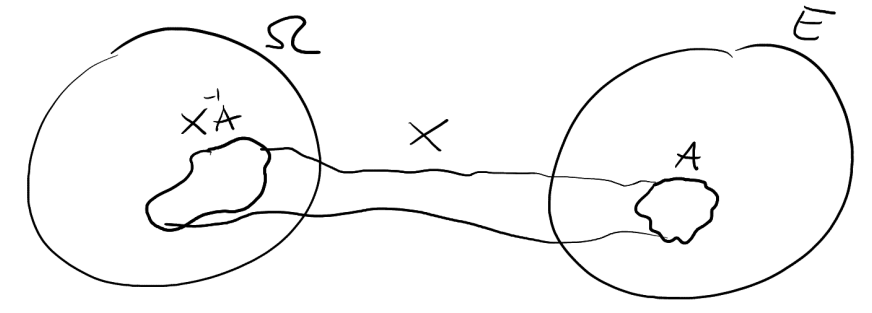
\includegraphics[width=0.8\linewidth]{screenshot001}
	\caption{this is an early reminder of the fact that I will take my own life very soon.}
	\label{fig:screenshot001}
\end{figure}
So if $X^{-1}A$ is measurable by $\pr$ then it is in $\mathscr{H}$: otherwise it is not in $\mathscr{H}$. So \[\pr(X^{-1}A)=\pr\left(\left\{\omega\in\Omega:X(\omega)\in A\right\}\right).\] The message is that I am interested/able to evaluate $\pr$ over the set only if what I am evaluating is indeed an event (which means: it belongs to $\mathscr{H}$\footnote{il lettore più arguto avrà notato che, a questo punto, il dio è ormai irrimediabilmente cane.}). If something is not in $\mathscr{H}$ get it off my fucking face man and kill yourself NOW\footnote{
		
\includegraphics[width=0.05\linewidth]{screenshot002}
}. This is the only restriction for a random variable. $E$ can be whatever we need it to be: a graph, a tree, your mom being absolutely \censor{torn apart} by me. But most of the times, we have $E=\R$ or $E=\R^d$ with respectively $\mathscr{E}=\mathscr{B}\footnote{Borel \sa. You don't know what a Borel \sa\; is? \url{https://en.wikipedia.org/wiki/Borel_set}}(\R)=\mathscr{B}_\R$ and $\mathscr{B}_{\R^d}$.
\begin{remark}
	The simplest random variables are indicator functions of events.
	Example: take $H\in\mathscr{H}$. Define the function
	\begin{align*}
		\indi_H&:\Omega\rightarrow\R\\
		\indi_H(\omega)&=\begin{cases}
			0 &\omega\not\in H\\
			1 &\omega\in H
		\end{cases}
	\end{align*}
\end{remark}
\begin{remark}
	A random variable is said to be \enf{simple} if it takes only finitely many values in $\R^d$.
\end{remark}
\begin{remark}
	A random variable is said to be \enf{discrete} if it takes only countably many values.
\end{remark}
\begin{definition}
	\enf{Distribution of a random variable}. Let $X$ be a random variable taking values in $(E,\mathscr{E})$ and let $\mu$ be the image of $\pr$ under $X$, that is,
	\[\mu(A)=\pr(X^{-1}A)=\pr(X\in A)=\pr\circ X^{-1}(A)\footnote{you would know this if you knew fucking measure theory I guess},\;A\in\mathscr{E}.\] Then $\mu$ is a probability measyre on $(E,\mathscr{E})$ and it is called \textbf{distribution of X}.
\end{definition}
So we map, by means of $X$, sets belonging to $\mathscr{E}$ into $\mathscr{H}$ and then evaluates this sets by means of the measure $\pr$. This is what we mean when we say that distributions are ultimately built with the probability measure and the random variable. Distribution is itself a measure!
\begin{remark}
	You should remember (LOL) that when we want to specify a measure on a $\sigma$-algebra, it's enough to do it on a \textit{p-system}\footnote{a p-system is a simpler object than a $\sigma$-algebra: it is simply a collection of sets closed under intersection} generating that $\sigma$ algebra: by means of the monotone class theorem we are then able to extend the measure to the $\sigma$-algebra. \\
	This means that to specity $\mu$ it is enough to specify it on a \textit{p-system} which generates $\mathscr{E}$. For example, consider $E=\overline{\R}, \mathscr{E}=\mathscr{B}_{\overline{\R}}$. Consider the collection of sets $[-\infty,x],\;x\in\R$ which is of course a p-system because it is closed under intersection. Moreover, this shit generates the Borel sigma algebra on $\overline{\R}$. \\If we want to define a distribution, that is a measure, it is enough to define it on this p-system. Imagine that we apply our distribution measure to one set of this p-system
	\[c(x)\footnote{because it is a function of $x$}=\mu\left([-\infty,x]\right)=\pr(X\leq x),\qquad x\in\R\] by the monotone class theorem. So we have now specified the measure on the p-system. The part $\pr(X\leq x)$ reminds us of the undergraduate times\footnote{I already wanted to kill myself at that time.}: it is a distribution function! This is what our professor did implicitly to avoid using measure theory\footnote{I have noticed that my life has not benefited in ANY form since I have been introduced to measure theory.}.
\end{remark}
\subsection{Functions of random variables}
Consider $X$, a random variable taking values in $(E,\mathscr{E})$ and consider further a measurable space $(F,\mathscr{F})$. Let $f:E\rightarrow F$ be a measurable function relative to $\mathscr{E}$ and $\mathscr{F}$\footnote{This basically means that this bitch won't do anything evil. The whole point of measure theory, $\sigma$ algebras and all other shit is to ensure everything behaves.}. This function should me measurable by means of $\pr$, otherwise we couldn't do anything useful with it. Consider the composition
\[Y=f\circ X\qquad\text{such that}\;Y(\omega)=f\circ X(\omega)=f\big(X(\omega)\big),\;\omega\in\Omega.\]
This composition is a random variable taking values in $(F,\mathscr{F})$ which comes from the fact that measurable functions of measurable functions are still measurable. 
\begin{definition}
	Consider two random variables $X,Y$ taking values in $(E,\mathscr{E})$ and $(F,\mathscr{F})$ respectively. Consider the pair
	\[Z=(X,Y):\Omega\rightarrow E\times F.\]
	Why would we want to call it $Z$? It's because, beside being a random vector, it is in turn a random variable:
	\[Z(\omega)=(X(\omega),Y(\omega)).\]
	Since $E\times F$ is a product space, we should attach it the product $\sigma$-algebra. So $Z$ is a random variable taking values in $E\times F$. 
\end{definition}
Note that the product space $E\times F$ is endowed with the \sa $\mathscr{E}\otimes\mathscr{F}$, that is the product \sa generated by the collection of all possible rectangles between $E$ and $F$. We frequently have to look to special cases like random vectors that must take values in measurable spaces for them to make sense. This measurable space is naturally generated by the product \sa (but it may be generated by other $\sigma$-algebras\footnote{Repeatedly inflicting painful kicks on my gonads.}!).
\begin{definition}
	We call \enf{joint distribution} of $X$ and $Y$ the distribution of $Z$. 
\end{definition}
This is interesting, since we know that this variable has the specific structure of a random vector: we identify the distribution of this vector as the joint distribution of its two coordinates\footnote{it eludes me how anyone could find this interesting. We have to think about the whole vector as being distributed like its components separately}. 
\begin{remark}
	The product \sa{} $\mathscr{E}\otimes\mathscr{F}$ is generated by the p-system of measurable rectangles.
\end{remark}
On the product space, it is enough to only specify it on this p-system.\par
Let denote with $\pi$ the joint distribution of $X,y$. It is sufficient to specify
\[\pi(A\times B)=\pr(X\in A, Y\in B)\qquad\every  A\in\mathscr{E},B\in\mathscr{F}.\]
We exploited the measurability of $X$ and $Y$
\begin{definition}
	Given the joint distribution $\pi$, consider sets $A\in\mathscr{E},B\in\mathscr{F}$. Then we call \enf{marginal distribution of $X$}
	\[\pr(X\in A)=\pi(A\times F)\qquad\;\every  A\in\mathscr{E}\]
	and we call \enf{marginal distribution of $Y$}
	\[\pr(Y\in B)=\pi(E\times B)\qquad\;\every  B\in\mathscr{F}.\]
\end{definition}
We call it distribution because it is actually a measure! So we can call it with the notation of measure
	\[\mu(A)=\pr(X\in A)=\pi(A\times F)\qquad\;\every  A\in\mathscr{E}\] and \[\nu(B)=\pr(Y\in B)=\pi(E\times B)\qquad\;\every  B\in\mathscr{F}.\]This actually means that the second coordinate is fixed in being the \underline{whole space} $F$. Think about integrating the second coordinate along the real line when doing marginal distributions... this is the same thing here.\\
Now that we have joint and marginal distributions, what is the next step\footnote{Abandoning myself in the sweet embrace of Death, methinks.}?
\begin{definition}
	Let $X,Y$ be \rv s taking values in $(E,\mathscr{E})$ and $(F,\mathscr{F})$ respectively and let $\mu$ and $\nu$ be their respective distributions. Then $X$ and $Y$ are said to be \enf{independent} if their joint distribution is the product measure formed by their marginals.
	\[\pr(X\in A,Y\in B)=\pr(X\in A)\pr(Y\in B)\qquad\every  A\in \mathscr{E},B\in\mathscr{F}.\]
	This also means that 
	\[\pi=\mu\nu\]
\end{definition}
Here the marginals do not interact with each other. This is true for two random variables but we need\footnote{No.} something more general.
\begin{definition}
Let $(X_1,X_2,\ldots,X_n)$ be a finite collection of random variables. The collection is said to be an \enf{independency} if the distribution of $(X_1,X_2,\ldots,X_n)$ is the product of $\mu_1,\mu_2,\ldots,\mu_n$ where $\mu_i$ is the distribution of $X_i$, for $i=1,\ldots,n$.
\end{definition}
Cynlar is stupid I wish him dead to be frank for this independecy shit. Independecy is not even an english word. What the fuck? Anyway, what about infinite collections?
\begin{definition}
	Let $(X_n)_{_n}$ be an infinite collection of \rv s. It is said to be an \enf{independency} if every finite sub-collection of it is an independecy.
\end{definition}
We now turn to stochastic processes\footnote{Please no.}! But first...
\subsection{Infinite product spaces}
Let $T$ be an arbitrary (countable or uncountable) set. We will think about this set as an "index" set. For each $t\in T$ consider the measurable $(E_t,\mathscr{E}_t)$. So we have a space for each index (plenty of measurable spaces hanging around). Consider a point $x_t$ in $E_t$ for each $t\in T$. The collection\footnote{We could consider it a function of $t$ but that wouldn't be exactly correct since each $t$ has a different measurable space. We may have the same space but it's not true in general... I am thrilled to say the least.} $(x_t)_{_{t\in T}}$. If  $(E_t,\mathscr{E}_t)=(E,\mathscr{E})$ then $(x_t)_{_{t\in T}}$ is actually a function of $T$ taking values on $(E,\mathscr{E})$. \\
The set $F$ of all possible functions $x=(x_t)_{_{t\in T}}$ is called the \enf{product space} $\left((E_t\mathscr{E}_t)\right)_{_{t\in T}}$.\\ This is the natural generalization of what we do when we construct product spaces, albeit with a different notation. Usually $F$ is denoted by $X_{t\in T}E_t$. But we know we also need a \sa...\\
A \enf{rectange} in $F$ is a subset of the form
\[\{x\in F:x_t\in A_t \;\every t\in T\}\]
Where $A_t$ differs from $E_t$ for only a finite number of $t$. So I want to consider subsets of $F$ (the space of functions) of the form above. I want only the functions $x$ in $F$ such that each coordinate belongs to $A_t$, a subset of $E_t$ for each $t\in T$. It seems that we have a restriction on all the coordinates... But this may bring to problems when we have an uncountable number of coordinates and therefore an uncountable number of restrictions. But we can says that if $A_t=E_t$ (the whole space) we don't apply any restriction. So in this case  $X_t$ belongs to $E_t$ so we can choose whatever $X_t$ we like. So only a finite number of coordinates are restricted while the other infinite ones are free to vary\footnote{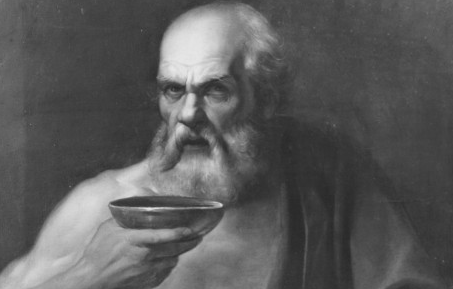
\includegraphics[width=0.08\linewidth]{screenshot003}$\rightarrow$ my honest reaction.
}. \par
The \sa{} generated by the collection of all measurable rectangles is denoted by 
\[\bigotimes_{t\in T}\mathscr{E}_t.\]
This is the product \sa{} in any infinite-dimensional space. So, the (natural) resulting measurable space in the end will be
\[\bigtimes_{t\in T}E_t,\bigotimes_{t\in T}\mathscr{E}_t.\] This is not in contrast with what we already know for finite product space, since these already have a finite number of restrictions. So this concept of rectangle, which can be a bit different from the one regarding the famous and well-tested geometrical shape\footnote{Oh thank god someone finally said it. I was starting to get scared.}, is not restricted on all the coordinates (like the shape\footnote{I swear to god.}) but only on a finite number of them. \\
We also have an alternative notation for this measurable space!
\[\bigotimes_{t\in T}(E_t,\mathscr{E}_t).\]
In the case that $(E_t,\mathscr{E}_t)=(E,\mathscr{E})\;\every t\in T$ the product space is denoted by
\[(E,\mathscr{E})^T\] or 
\[(E^T,\mathscr{E}^T)\]
These are not real powers but it's just notation... Anyway these are all different notations to indicate the infinite product space with the product \sa{} built upon the p-system which is the collection of all possible rectangle defined in the way we saw above\footnote{NO I WON'T USE LABELS AND NUMBERED EQUATIONS.}.
\subsection{Stochastic processes}
\begin{definition}
	Let $(E,\mathscr{E})$ be a measurable space and consider an index set $T$ (as before, an arbitrary set countable or uncountable).\\
	Let also $X_t$ be a \rv{} taking values in $(E,\mathscr{E})$. Then the collection of those random variables $(X_t)_{_{t\in T}}$ is called a \enf{stochastic process} with state space $(E,\mathscr{E})$ and parameter set $T$.
\end{definition}
Note that there is no mention about time here. Just think about the index set, which indexes the stochastic process. If we interpret $T$ as time then we have the most common interpretation of stochastic processes. But it could also be space (imagine $\R^2$) or your mom being \censor{fucked hard}. Anyway the most natural interpretation is time.\par
Now take a $\omega\in\Omega$ and evaluate all these \rv s on the same $\omega$. What we get is
\[t\mapsto X_t(\omega)\]
which is a function from $T$ to $(E,\mathscr{E})$. So if we see it as a function of $t$ for each $\omega$ we get a function which is an element of $E^T$. So what is a stochastic process, to sum it up? It's just a random variable taking values in the infinite product space $E^T$. That's why it is a problematic object: it's because mathematicians deserve to experience the sadness and evil they unleashed upon the world. Ever noticed how similar the words "measurable" and "miserable" are? I didn't think so. 
\begin{figure}[H]
	\centering
	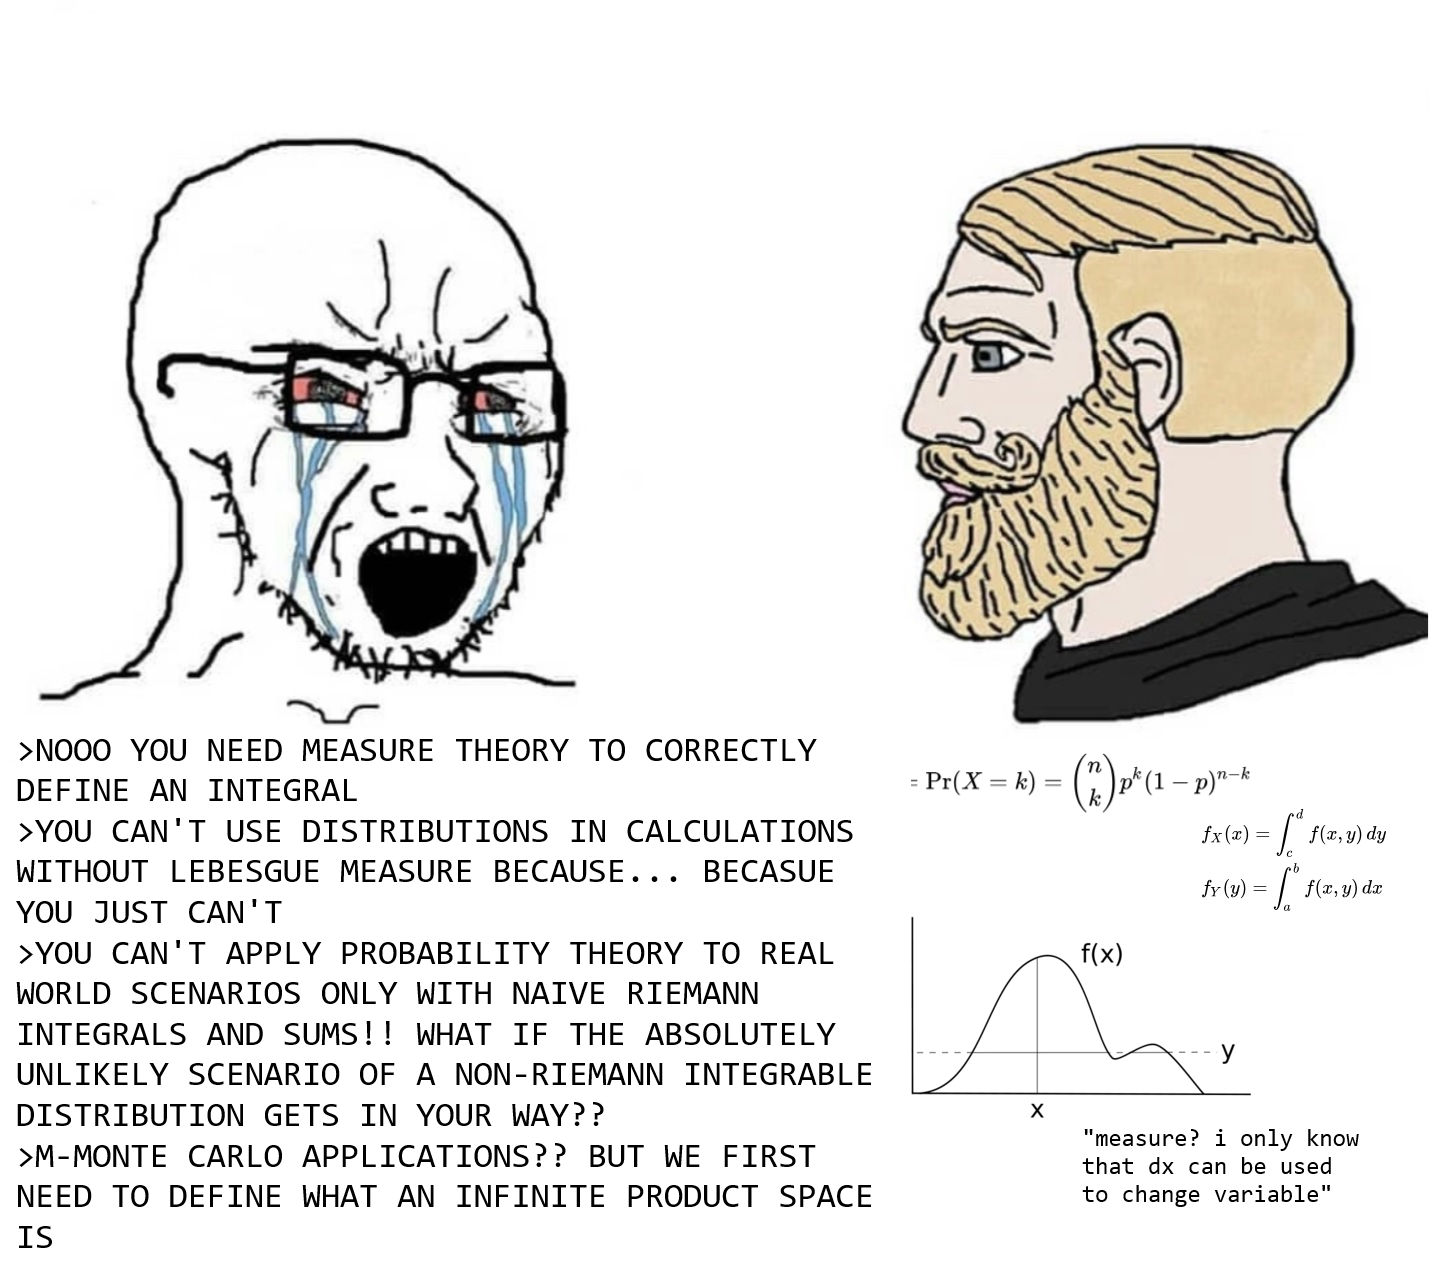
\includegraphics[width=0.6\linewidth]{ILMEMINO}
	\caption{I'm sorry but here you're the soyjack and I'm the chad.}
	\label{fig:ilmemino}
\end{figure}
Yeah technically more structure helps us modeling real phenomena more accurately but who the FUCK cares. 
\subsection{Example of random variables}
Consider some examples of simple random variables:
\begin{example}
	\enf{Poisson \rv s.}\\
	This \rv{} takes vales in $\N$ (it's a one dimensional \rv{}). We consider the power set of $\N$\footnote{Subset of all subsets of $\N$.}. We know that power sets \textit{are} \sa s that we can use (but we could encounter some trouble with uncountable elements, for which we would need smaller \sa s\footnote{No one really cares, not even Federico Polito.}).\\
	What is the distribution of this \rv{}?
	\begin{align*}
	\mu(A)=\pr(X\in A)&=\sum_{n\in A}\pr(X=n)\qquad A\subset\N\\
	\text{with } \pr(X=n)&=e^{-c}\frac{c^n}{n!}, \;n\in\N,\;c>0.
	\end{align*}
	So imagine we have this kind of random variable. We consider a subset of the natural number and we want to evaluate the measure of this subset that we chose. We know that we define the \rv{} by defining the distribution. For each $n$ we get a number $e^{-c}\frac{c^n}{n!}$. Another interesting implication is that \[\sum_{n\in A}\pr(X=n)=\sum_{n\in\N}\delta_n(A)\pr(X=n)\] where $\delta_n(A)$ is the \enf{Dirac measure} sitting at $n$. So, $n$ is a parameter and 
	\[\delta_n(A)=\begin{cases}
		1 &n\in A\\
		0 &n\not\in A
	\end{cases}.\] The Dirac measure is similar to the indicator function (they behave basically in the same way) but the difference is that this one is a \textit{measure} and the latter is a \textit{function}. The Dirac measure has $n$ as a parameter, while the indicator function has the set as a parameter ($\indi_A(n)$).
\end{example}
\begin{example}
	\enf{Exponential \rv{}}\\
	This random variable is again one-dimensional but this time this random variable is \textit{absolutely continuous}. What does it mean? It actually means that the variable is absolutely continuous with respect to the Lebesgue measure\footnote{'tacci tua.}. This is evident when we write down the distribution.\\
	Consider a \rv{} taking values in $\R_+$ and further consider $\mathscr{B}_{\R_+}$. We have
	\[\mu(\dif x)=\underbracket{\dif x}_{\mathclap{Leb(\dif x)}}ce^{-cx},\qquad c>0,\;x\in\R_+\]
	WHY ON EARTH did we write $\dif x$ instead of just $x$? That's a good question. $\dif x$ stands for the Lebesgue measure of $\dif x$\footnote{Why? I will kill my own self.}. The second part of the equation ($ce^{-cx}$) is the density part and, being a continuous function, it implies that the distribution is continuous with respect to the Lebesgue measure\footnote{Really??}. So $p(x)=ce^{-cx},\;d\in\R_+$ is the density relative to $\mu$.
\end{example}
It is interesting\footnote{Debatable claim.} to see that also discrete random variable turns out to be absolutely continuous... But not with respect to the Lebesgue measure. To exact, discrete \rv s are absolutely continuous with respect to the \textit{counting} measure.
\end{document}